\documentclass[xcolor=dvipsnames]{beamer}
\usepackage{graphicx}
\usepackage{xcolor}
\usepackage{tikz}
\usepackage{multicol}
\usepackage[absolute, overlay]{textpos}
\usepackage{fontspec}
\setsansfont[
ItalicFont=Roboto-LightItalic.ttf
]{Roboto Light}
\usepackage{tcolorbox}

\graphicspath{{fig/}}


% define themes
\usecolortheme{dolphin}

% change text to offblack
\definecolor{almostblack}{HTML}{262626}
\setbeamercolor{normal text}{fg=almostblack}

% macros
\newcommand{\trento}{T\raisebox{-0.5ex}{R}ENTo}

\definecolor{theme}{RGB}{90,122,163}
\usecolortheme[named=theme]{structure}

\makeatletter
\setbeamertemplate{frametitle}{
  \ifbeamercolorempty[bg]{frametitle}{}{\nointerlineskip}%
  \@tempdima=\textwidth%
  \advance\@tempdima by\beamer@leftmargin%
  \advance\@tempdima by\beamer@rightmargin%
  \begin{beamercolorbox}[sep=0.3cm,left,wd=\the\@tempdima]{frametitle}
    \vbox{}\vskip-2ex%
    \if@tempswa\else\csname beamer@fteleft\endcsname\fi%
    \strut\insertframetitle\strut\par%
    {%
      \ifx\insertframesubtitle\@empty%
      \else%
      {\usebeamerfont{framesubtitle}\usebeamercolor[fg]{framesubtitle}\insertframesubtitle\strut\par}%
      \fi
    }%
    \vskip.45ex%
    \hrule %height .6pt%
    \vskip-1.45ex%
    \if@tempswa\else\vskip-.3cm\fi%
  \end{beamercolorbox}%
}
\makeatother

% clean up footer
\beamertemplatenavigationsymbolsempty
\setbeamertemplate{footline}[frame number]

%inner theme
\useinnertheme{rectangles}
\setbeamertemplate{itemize item}{\raise.30ex\hbox{\vrule width .80ex height .80ex}}
\setbeamertemplate{itemize subitem}{\raise.35ex\hbox{\vrule width .70ex height .70ex}}

%\title{Determining QGP initial conditions and medium properties via Bayesian model-to-data analysis}
\author{J.S. Moreland, J.E. Bernhard, S.A. Bass}
\date{\today}


\begin{document}

\section{Title}

\usebackgroundtemplate{%
\tikz[overlay,remember picture] \node[opacity=0.4, at=(current page.center)] {
   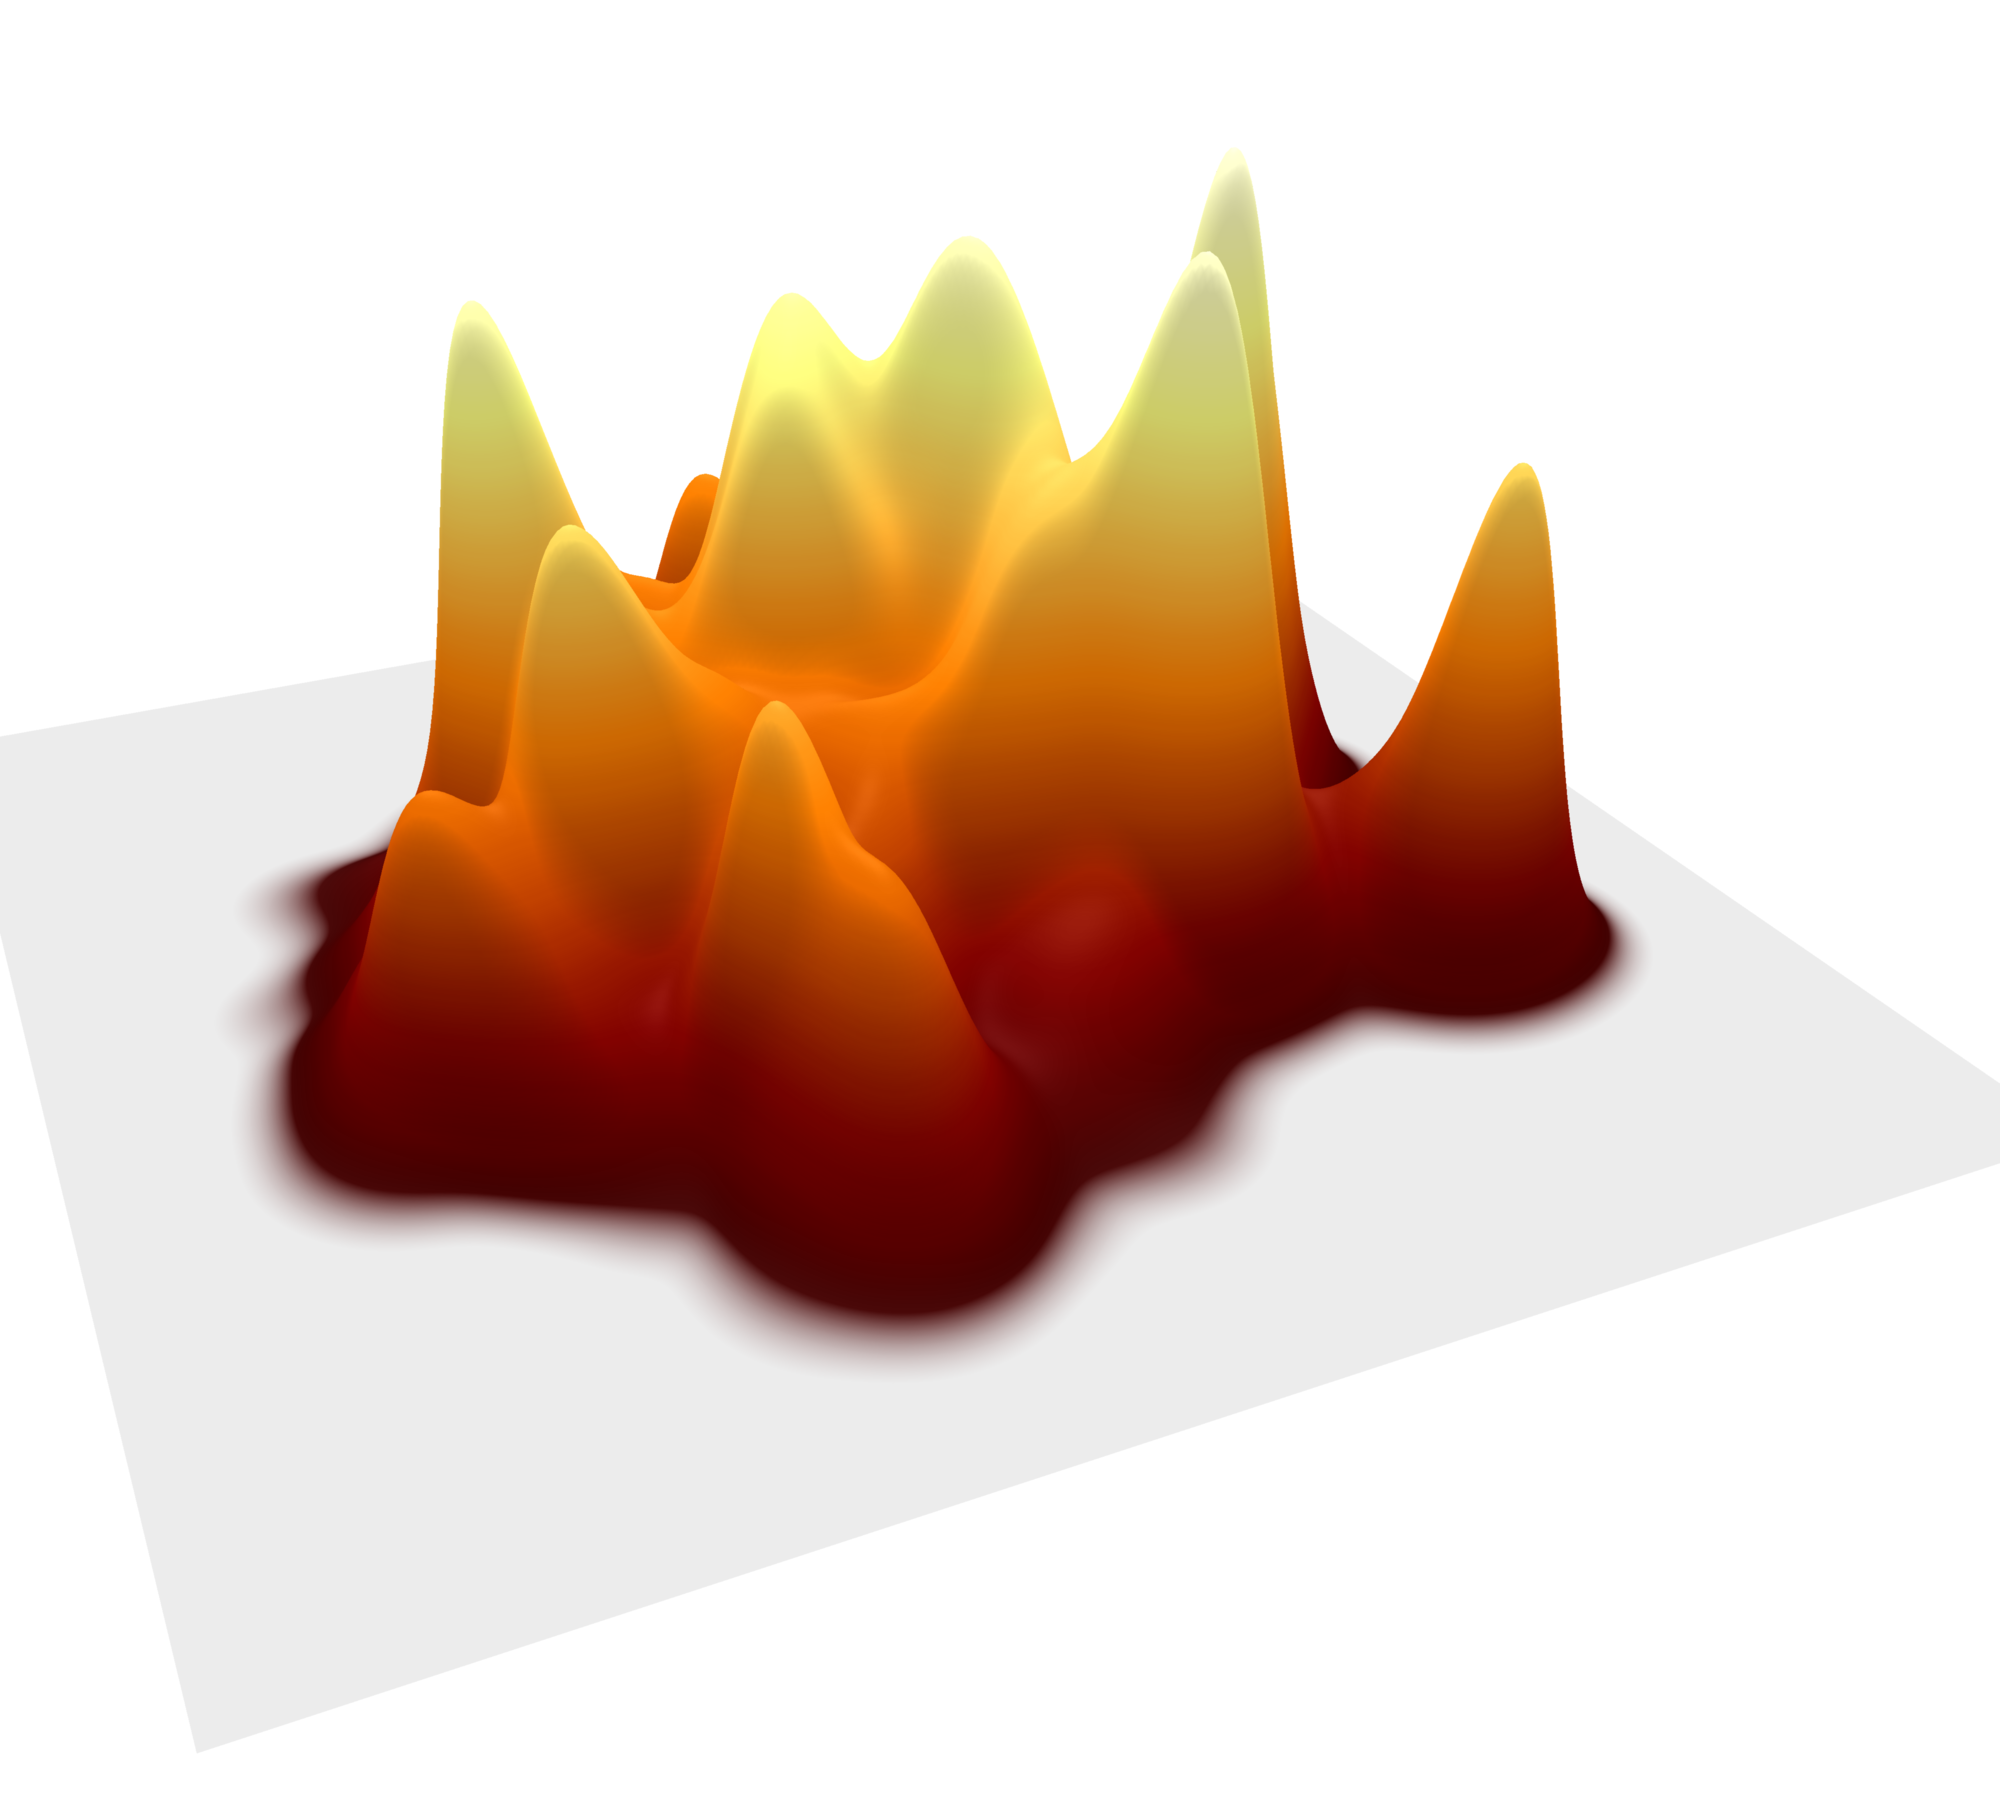
\includegraphics[width=\paperwidth]{trento2}};
}

\frame[plain,noframenumbering]{
  \begin{tikzpicture}[remember picture,overlay]
    \coordinate (middle) at (current page.center);
    \def\sep{.028\paperwidth}
    \def\extra{.6em}
    \node[rectangle, fill=theme, align=center, anchor=center, yshift=2.75cm, fill opacity=0.08, text opacity=1] at (middle) {
      \color{theme} \Large
      Determining QGP initial conditions and medium\\
      \color{theme} \Large
      properties via Bayesian model-to-data analysis
    };
    \node[align=center, anchor=center, yshift=1. cm] at (middle) {
      \insertauthor \\[\extra]
      Initial Stages~$\vert$~\insertdate
    };
    \node[align=center, anchor=center, yshift=-3 cm] at (middle) {
      
\includegraphics[height=1.2cm]{qcdlogo} \hspace{0.2 cm} \hspace{0.2 cm}
      
\includegraphics[height=1.cm]{ssgf} \vspace{0.2 cm} \\
      \tiny Funding provided by DOE Stewardship Science Graduate Fellowship
    };
  \end{tikzpicture}
}

\usebackgroundtemplate{}

\begin{frame}{Motivation: why study the QGP initial conditions?}
    \bigskip
    QGP initial state and its various roles {\scriptsize [Angerami IS15' Napa]}: \\
    \begin{itemize}
        \item The initial conditions are interesting in their own right. \\
        \medskip
        One ultimately seeks a first principles description of initial entropy deposition and thermalization. \\
        \medskip
        \item The initial conditions are a "nuissance parameter" in hydrodynamic simulations. We need them to extract transport properties, e.g.\ ~$\eta/s$, ~$\zeta/s$, ~$\hat{e}$, ~$\hat{q}$, etc.     
    \end{itemize}
    \medskip
    Deriving QGP IC from first principles is \emph{challenging}...\\ 
    \medskip
    \begin{tcolorbox}[width=\textwidth, colback=theme!10, colframe=theme!0]
        Can we determine the IC from experiment without detailed knowledge of the initial stages of the collision?
        \medskip \centering \\
        What can we learn with such knowledge?
    \end{tcolorbox}
\end{frame}

\begin{frame}{Deconstructing initial condition models}
    Start by defining local entropy (or energy) deposition in the eikonal approximation,\\ 
    \begin{equation*}
        \frac{dS}{d^2r_\perp dy} \biggr \vert_{\sqrt{s_{NN}}} = \text{Norm} \cdot f(T_\text{part, A}, T_\text{part, B})
    \end{equation*}\\
    \vspace{0.1 cm}
    
    Mapping should only respect matter \underline{in the cross section} and hence,\\
    \begin{equation*}
        T_\text{part}(\vec{x}) = \sum\limits_{i=1}^{N_\text{part}} T_p(\vec{x} - \vec{x}_i)
    \end{equation*}
    In general, the normalization and mapping $f(T_\text{part, A}, T_\text{part, B})$ could have some dependence on $\sqrt{s_{NN}}$.
\end{frame}

\begin{frame}{Thinking of boost-invariant IC models as a surface}
\end{frame}

\begin{frame}{Hybrid transport model}
    Hybrid model \\
    \begin{itemize}
        \item iEBE-VISHNU model
        \item HotQCD equation of state
        \item UrQMD hadronic afterburner
    \end{itemize}
\end{frame}

\begin{frame}{\trento\ initial condition model \quad{\scriptsize Phys.\ Rev.\ C {\bf 92}, no.\ 1, 011901 (2015)}}
    \vspace{.6 cm}
    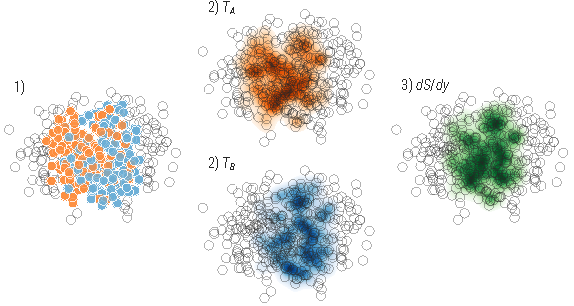
\includegraphics{schematic} \\
    \begin{enumerate}
        \scriptsize
        \setbeamercolor{item projected}{bg=theme!40, fg=almostblack}
        \item Calc participants: $P_\text{coll}(b) = 1 - \exp[-\sigma_{gg} T_{pp}(b)]$, \quad $\int 2 \pi\, b\, db\, P_\text{coll}(b) = \sigma_\text{NN}^\text{inel}$ \\ \vspace{0.1 cm}
        \item Build participant density: $T_A(x,y) = \sum\limits_{i=1}^{N_{\text{part},A}} \gamma_i T_p(x-x_i, y-y_i)$, \quad $\gamma \sim \Gamma(k, 1/k)$ \\
        \item Parameterize entropy deposition w/ generalized mean: $dS/dy \propto \bigg(\frac{T_A^p + T_B^p}{2} \bigg)^{1/p}$
    \end{enumerate}
\end{frame}

\begin{frame}{Efficacy of the genealized mean}
    \vspace{0.4 cm}
    \begin{columns}
        \begin{column}{0.5\textwidth}
            \includegraphics{thickness} 
        \end{column}
        \begin{column}{0.5\textwidth}
            \centering
            \begin{itemize}
                \item dog
                \item cat
                \item monkey
            \end{itemize}
        \end{column}
    \end{columns}
    \vspace{0.2 cm}
    \begin{columns}
        \begin{column}{\textwidth}
            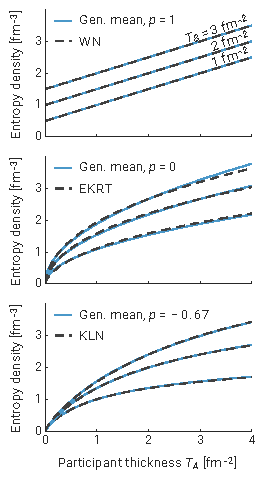
\includegraphics{cgc_compare} \\
            \scriptsize
            The generalized mean can be tuned to replicate the behavior of many CGC calculations
        \end{column}
    \end{columns}
\end{frame}

\begin{frame}{Calibrating the model}
    \vspace{0.4 cm}
    \begin{itemize}
        \scriptsize
        \item Top row: run model ($\times10^4$ events) at each design point ($\times300$ parameter sets)
        \vspace{0.2 cm}
        \item Bottom row: emulator predictions for 100 samples from the posterior distribution
    \end{itemize}
    \vspace{0.2 cm}
    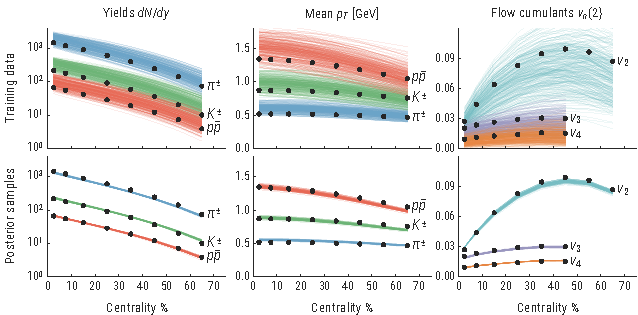
\includegraphics{observables_plot}
\end{frame}

\begin{frame}{Running the model with high-likelihood parameters}
    \vfill
    \centering
    \begin{columns}
        \begin{column}{0.4\textwidth}
            Choose high likelihood \\model parameters
        \end{column}
        \begin{column}{0.6\textwidth}
            \begin{tabular}{lllll}
                \multicolumn{2}{c}{Initial condition} & & \multicolumn{2}{c}{QGP medium} \\
                \noalign{\smallskip}\hline\noalign{\smallskip}
                norm & 120.          &&  $\eta/s$ min   & 0.08       \\
                $p$  & 0.0           &&  $\eta/s$ slope & 0.85 GeV$^{-1}$   \\
                $k$  & 1.5           &&  $\zeta/s$ norm & 1.25       \\
                $w$  & 0.43 fm       &&  $T_\text{sw}$  & 0.148 GeV  \\
            \end{tabular}
        \end{column}
    \end{columns}
    \vspace{0.5 cm}
    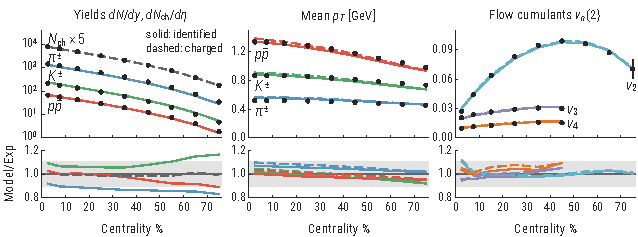
\includegraphics{mode_observables} \\
    \vspace{0.2 cm}
    No emulator! Results represent actual hydro + UrQMD calculations!
\end{frame}

\begin{frame}
    \begin{flushleft}
        \only<1->{\includegraphics{posterior_identified}}
    \end{flushleft}

    \begin{textblock}{10}(3.2, 1.2)
        \only<3->{\textcolor{gray}{entropy normalization}}
        \only<1,2>{entropy normalization}
    \end{textblock}
    
    \begin{textblock}{10}(4.3, 3)
        \only<2,4->{\textcolor{lightgray}{entropy normalization}}
        \only<1,3>{entropy generalized mean}
    \end{textblock}
    
    \begin{textblock}{10}(6.0, 4.8)
        \only<2-3,5->{\textcolor{lightgray}{nucleon Gamma fluctuation}}
        \only<1,4>{nucleon Gamma fluctuation}
    \end{textblock}
    
    \begin{textblock}{10}(6.6, 6.6)
        \only<2-4,6->{\textcolor{lightgray}{Gaussian nucleon width [fm]}}
        \only<1,5>{Gaussian nucleon width [fm]}
    \end{textblock}
    
    \begin{textblock}{10}(8.0, 8.4)
        \only<2-5,7->{\textcolor{lightgray}{$\eta/s$ min at critical temperature}}
        \only<1,6>{$\eta/s$ min at critical temperature}
    \end{textblock}
    
    \begin{textblock}{10}(10.0, 10.2)
        \only<2-6,8->{\textcolor{lightgray}{$\eta/s$ slope [GeV$^{-1}$]}}
        \only<1,7>{$\eta/s$ slope [GeV$^{-1}$]}
    \end{textblock}
    
    \begin{textblock}{10}(11.5, 12)
        \only<2-7,9->{\textcolor{lightgray}{$\zeta/s$ normalization}}
        \only<1,8>{$\zeta/s$ normalization}
    \end{textblock}
    
    \begin{textblock}{10}(12.5, 13.6)
        \only<2-8>{\textcolor{lightgray}{hydro-to-UrQMD \\
        switching temp [GeV]}}
        \only<1,9>{hydro-to-UrQMD \\
        switching temp [GeV]}
    \end{textblock}
\end{frame}

\begin{frame}
    \includegraphics{nch_per_npart_2}
\end{frame}

\begin{frame}{Conclusions}
Yields, mean $p_T$ and flows impose strong constraints on IC. \\
Entropy  deposition mimic'd by $dS/dy \sim \sqrt{T_A T_B}$ \\
Data strongly prefers small nucleon width $w \approx 0.43$ fm! \\
A+A collisions weakly sensitivie to p+p mult.\ fluctuations \\
Prefered initial conditions similar to EKRT, IP-Glasma \\


\end{frame}
\end{document}
